\newpage
\subsection{LoRa}
LoRa is a wireless communication protocol that is designed for long-range, low-power, and low-data-rate applications. LoRa is based on chirp spread spectrum modulation (CSS) technology, which enables long-range communication with low power consumption, making it suitable for IoT devices that need to transmit data over long distances while consuming minimal power.

\begin{figure}[!h]
    \centering
    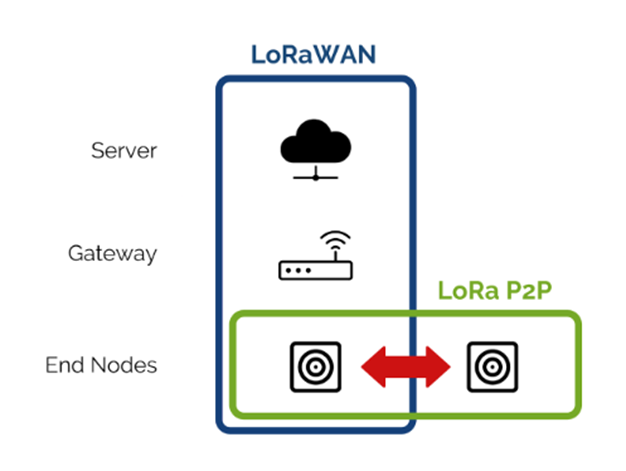
\includegraphics[width=0.8\textwidth]{\currfiledir/figures/lora_P2P.png}
    \caption{LoRa WAN and LoRa P2P scheme}
\end{figure}

LoRa is primarily designed for long-range communication between IoT devices and gateways using a star network topology. However, it is possible to use LoRa for peer-to-peer (P2P) communication between two LoRa devices without the need for a gateway or network server.
This type of communication becomes important and applicable because the remote monitoring system, to which the LoRa protocol will be applied, is located in a forest. Where there is no internet connection.


%3.6.1	Analysis and expressions of needs for LoRa
\subsubsection{Analysis and expressions of needs for LoRa}
The analysis and expression of needs would involve identifying the specific requirements for LoRa. For this, it is considered two main needs. The first is to establish communication between the transmitter and the receiver. The second is to cover a distance greater than or equal to 10 km. The goal is to send data via LoRa protocol, obtained by the sensors connected to the remote monitoring system, directly to the site where researchers will be able to analyse the information about its operation.

\newpage
%3.6.2	Use case for LoRa
\subsubsection{Use case for LoRa}
The system would then be placed in the desired location within the forest. For this reason, LoRa peer-to-peer communication will be used, as there is no internet connection in the location mentioned. All operating data obtained by the monitoring system will be passed to the LoRa transmitter via the microcontroller. With this, the data sent should reach the receiver located at a distance of 10 km or more. Finally, with the communication effected, the researchers will be able to analyze the operating conditions of the system.  In our case, the architecture is organized like this:
\begin{figure}[!h]
    \centering
    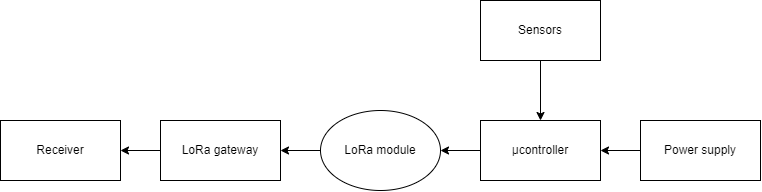
\includegraphics[width=1\textwidth]{\currfiledir/figures/lora_diagram.png}
    \caption{LoRa architecture diagram}
\end{figure}

\newpage
%4.6.4	Technical constraints
\subsubsection{Technical constraints}
%Graph presenting the different elements exercising constraints on the LoRa
\begin{figure}[!h]
    \centering
    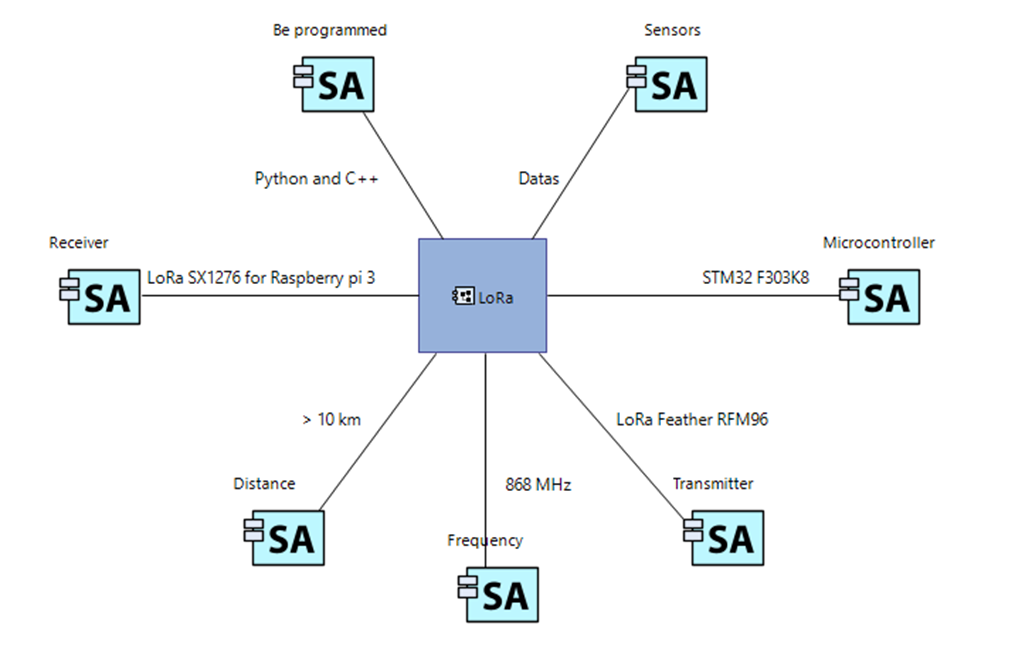
\includegraphics[width=0.90\textwidth]{\currfiledir/figures/lora_constraint.png}
    \caption{Graph presenting the different elements exercising constraints on the LoRa}
\end{figure}

%bold text "a"
\noindent\textbf{Sensors:} The sensors will be the source of the monitoring system's operational data, which will be sent for transmission via LoRa protocol.\\

\noindent\textbf{Microcontroller:} The microcontroller STM32 F303K8 will pass the data obtained from the sensors to the LoRa transmitter, so that this information can be sent to the receiver.\\

\noindent\textbf{Transmitter:} As a transmitter, the LoRa Feather RFM96 will be used, which will send the obtained data to the receiver.\\

\noindent\textbf{Frequency:} The frequency on which the LoRa communication will take place is 868 MHz.\\

\noindent\textbf{Distance:} Sending data must pass over a distance of 10 km or more.\\

\noindent\textbf{Receiver:} The Lora SX1276 connected to the raspberry pi 3 will be used as a receiver, which will act as a gateway allowing researchers to retrieve data from the monitoring system.\\

\noindent\textbf{Be programmed :}  In order for communication to take place, a code for sending data, in C++ language will be written in the LoRa transmitter connected to the microcontroller. For the receiver, a code in python will be written for retrieving the sent data.

%lora transmitter
\subsubsection{LoRa transmitter}
As transmitter the LoRa RFM95W module is used, which is connected to the STM32. The RFM95W module is based on the Semtech SX1276 chip, which is a high-performance, low-power LoRa transceiver. It operates in the 868 MHz and 915 MHz frequency bands, and provides a range of up to 5-10 km in open areas, depending on the transmit power and other environmental factors.
\begin{figure}[!h]
    \centering
    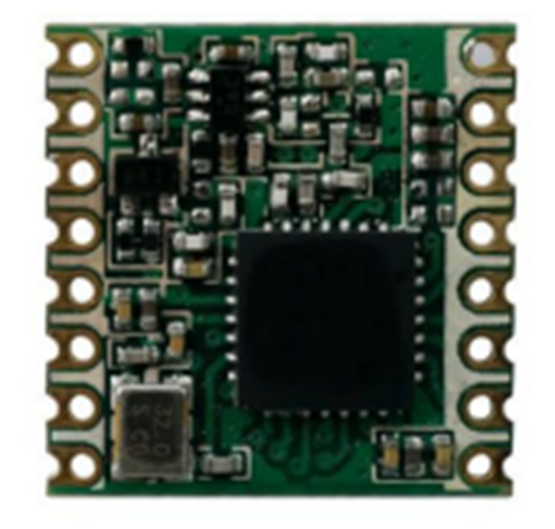
\includegraphics[width=0.50\textwidth]{\currfiledir/figures/RFM95W.png}
    \caption{LoRa RFM95W}
    \cite{RFM95W}
\end{figure}

Before configuring the LoRa module to act as a transmitter, it was necessary to connect a wire to the component in order to obtain an antenna. The size of the wire varies according to the transmission frequency. In this case for a frequency of 868 MHz, according to the manufacturer's website, the wire size is 8.2 cm. Because of this it was used.\\
Next, the Arduino IDE was used to configure and implement the C++ code, available for analysis in the appendix, for sending data via LoRa. The code was written with the help of existing Arduino libraries and forums on the subject available on the internet.

\newpage
%lora receiver
\subsubsection{LoRa receiver}
As receiver, the LoRa SX1276/ GPS Hat for Raspberry will be used. In this sense, the Raspberry pi 3 connected to the LoRa will have access to the received information. The currently available module for the project already has an uFL antenna.

\begin{figure}[!h]
    \centering
    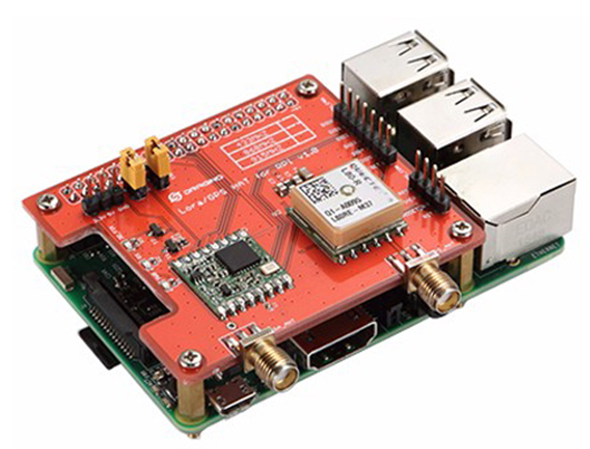
\includegraphics[width=0.60\textwidth]{\currfiledir/figures/lora_hat.png}
    \caption{LoRa/GPS HAT for Raspberry}
    \cite{Lora}
\end{figure}

The data received by Raspberry is automatically stored in a database available in a libre office Calc folder. This way, the user can have easy access to the system state.
For the Raspberry to work as a data receiver, it was necessary to configure it to enable some functions and update and download specific libraries for the LoRa SX1276. With this done, a program was written in python, available for analysis in the appendix, to receive the data. The data received by Raspberry is automatically stored in a database available in a libre office Calc folder. This way, the user can have easy access to the system state.\\

\begin{figure}
    \centering
    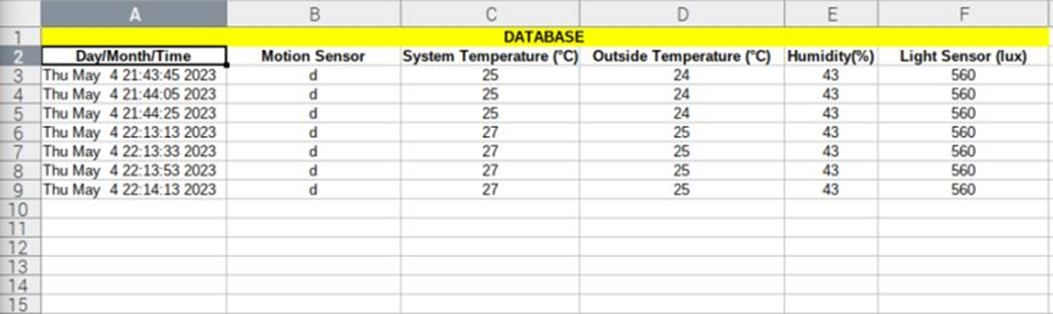
\includegraphics[width=0.8\textwidth]{\currfiledir/figures/lora_database.png}
    \caption{Sensors database}
\end{figure}

The database records the date and time each information is received. For the motion sensor, the letter "d" means that there is receiving data, if the system eventually moves, data about the movement will be sent, and letter "m" will appear in the database, indicating movement.


% \subsubsection{Tests to be performed for the LoRa communication system}
% The functional testing of the LoRa system will focus on two main aspects: communication between transmitter and receiver, and the maximum distance over which data can be sent.\\
% For the first one, through programming, a simple data transmission should be performed to the receiver using the LoRa transmitter. In this sense, a check of the received data should be made to see that no information has been lost.\\
% With the communication established, the test of the range of the transmission signal was performed. The transmitter was positioned on the second floor of the Les Roses building at approximately 230 m from the receiver, in the Fablab, at Polytech Vinci. An image representing the location and distance between the transmitter and receiver is shown below:\\
% \newpage
% \begin{figure}[!h]
%     \centering
%     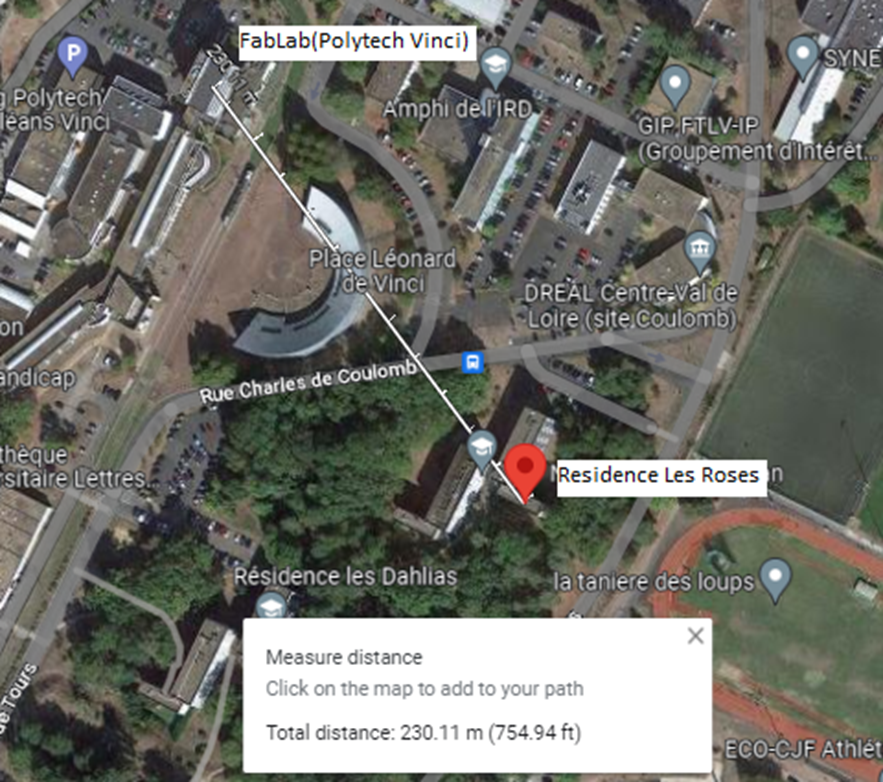
\includegraphics[width=0.60\textwidth]{\currfiledir/figures/map.png}
%     \caption{Location and distance between the transmitter and receiver.}
% \end{figure}

% Although the data was received in Raspberry, the signal was weak. The signal information is listed below:\\
% \tab •	Packet RSSI: -97\\
% \tab •	RSSI: -96\\
% \tab •	SNR: -8\\
% The factors that may have influenced this result are related, above all, to the transmission power and to the urban area noise that interferes with the signal quality.\\
% First, the antenna used for transmission is an 8.2 cm wire connected to the microcontroller. By replacing it with a more powerful model, it will be possible to send the signal over a longer distance.\\
% Next, the place where the transmission was made was not exactly the highest point of the building.\\
% Besides these factors, there is the fact that the signal suffers interference from urban noise, which affects the signal quality.\\
% Finally, in the transmission settings, the signal was sent with a Spreading factor SF=7, and it is possible to increase it up to a value of SF=12.\\
% Moreover, after these measures are put in place, the maximum distance at which it is possible to send this information from the transmitter to the receiver will be tested again. Here it is worth pointing out that it will be necessary to perform this test in a place where the signal transmission is not so affected by noise, such as in the city. Preferably a place where the conditions can be approximated to the place where the LoRa system will be used.\\
% Next, with the communication already established, the sensors will be integrated into the system and their information, regarding temperature and humidity for example, should be read at the receiver with the Raspberry's help.